\chapter{Berry's phase-based Unruh effect detection at lower accelerations\footnote{E. Mart\'in-Mart\'inez, I. Fuentes and R. B. Mann. arXiv:1012.2208}} \label{BerryPh}

\markboth{Chapter 13. Berry's phase-based Unruh effect detection}{\rightmark}

Finding indisputable corroboration of the Unruh effect is one of the main experimental goals of our time \cite{experiments,Crispino}. The effect is one of the best known predictions of quantum field theory incorporating general relativity. However, its  very existence has been object of a lengthy controversy  \cite{sceptic}.  Its observation would provide not only an end to such discussion but also experimental support for the Hawking radiation and black hole evaporation given the deep connection between these phenomena \cite{Hawking,Davies}.  Detection of the Unruh effect would therefore have an immediate impact in many fields such as astrophysics \cite{Astronature,Astrophysics}, cosmology \cite{Cosmo}, black hole physics \cite{Bholes}, particle physics \cite{Base}, quantum gravity \cite{Qg} and relativistic quantum information \cite{Alsingtelep,Alicefalls,QI}. 


As seen along this thesis, in the Unruh effect \cite{Unruh0,Crispino} the vacuum state of a quantum field corresponds to a thermal state when described by uniformly accelerated observers. Its direct detection  is unfeasible with current technology since the Unruh temperature is smaller than 1 Kelvin even for accelerations
as high as $10^{21}$ $\text{m}/\text{s}^2$.  Sustained accelerations higher than $10^{26}$ $\text{m}/\text{s}^2$ are required in the best proposal so far  to diretcly detect the effect \cite{ChenTaj,Crispino}.

Efforts on finding evidence of the Unruh and Hawking effects also include proposals in analog systems such as fluids \cite{Unruhan}, Bose-Einstein condensates \cite{garay}, optical fibers \cite{optfib}, slow light \cite{slowlight},  superconducting circuits \cite{supercond} and trapped ions \cite{ions}.  Even in such systems,  analog effects produce temperatures of the order of nanokelvin that remain difficult to detect.

 In this chapter we show that the state of an accelerated detector coupled to the field acquires a Berry phase \cite{Berryoriginal,aharonov} due to its movement in spacetime. This geometric phase, which is a function of the detector's trajectory, encodes information about the Unruh temperature and it is observable for accelerations as low as $10^{17}$ $\text{m}/\text{s}^2$. Such acceleration must be sustained only for a few nanoseconds. Our results enormously simplify the challenge of measuring the Unruh effect with present technology since producing extremely high accelerations and measuring low temperatures were the main obstacles involved in its detection and we reduce the accelerations needed by a factor $10^9$.  The results presented here are independent of specific experimental implementations; however, we propose a possible scheme for the detection of this phase.

Interestingly, it has gone unnoticed that Berry's phase can be employed to detect the Unruh effect. Berry showed that an eigenstate of a quantum system acquires a phase, in addition to the usual dynamical phase, when the parameters of its Hamiltonian are varied in a cyclic and adiabatic fashion \cite{Berryoriginal}.  In the case of a point-like detector interacting with a quantum field, the movement of the detector in spacetime produces, under certain conditions, the cyclic and adiabatic evolution that gives rise to Berry's phase. In what follows we will show that the Berry phase for an inertial detector
differs from that of an accelerated one.  This difference arises due to the Unruh effect: one detector interacts with the vacuum state while the second interacts with a thermal state. The Berry phase of an accelerated detector depends on the Unruh temperature. Surprisingly, we find that this phase is observable for detectors moving with relatively low accelerations, making the detection of the Unruh effect  accessible with current technology.

\section{The setting}

In our analysis, we consider a massless scalar field in the vacuum state from the perspective of inertial observers moving in a flat ($1+1$)-dimensional spacetime. The same state of the field corresponds to a thermal state from the perspective of uniformly accelerated observers.  The temperature of this thermal state is the so-called Unruh temperature $T_U=\hbar a / (2\pi c \omega)$ where $a$ is the observer's acceleration.
\begin{figure}[h]
\begin{center}
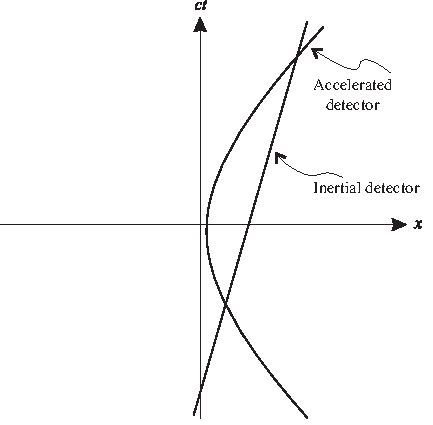
\includegraphics[width=.70\textwidth]{traj}
\caption{Trajectories for an inertial and accelerated detector.}
\label{setup}
\end{center}
\end{figure}
In order to show evidence of this effect we consider a point-like detector endowed with an internal structure which couples linearly to a scalar field $\hat\phi(x(t))$ at a point $x(t)$ corresponding to the world line of the detector. The interaction Hamiltonian is of the form $H_I\propto  \hat m(t) \hat \phi(x(t))$ where $\hat m(t)$ is the monopole momentum of the detector. We have chosen the detector to be modeled by a  harmonic oscillator with frequency $\Omega_b$. In this case the operator $\hat m\propto (b^\dagger + b)$ corresponds to the detector's position quadrature where $b^{\dagger}$ and $b$ are ladder operators .

 Considering that the detector couples only to a single mode of the field with frequency  $|k|=\Omega_a$, the field operator takes the form
 \begin{equation}
 \hat\phi(x(t))\approx\hat\phi_k(x(t))\propto \left[a\, e^{i(kx-\Omega_a t)}+a^\dagger\, e^{-i(kx-\Omega_a t)}\right],
 \end{equation}
  where $a^{\dagger}$ and $a$ are creation and anihilation operators associated to the field mode $k$.  The Hamiltonian is therefore
\begin{equation}\label{goodham2}
H_{T}=\Omega_a\, a^\dagger a +\Omega_b\, b^\dagger b+ \lambda (b+b^\dagger)(a^\dagger e^{i\varphi}\!+ a\, e^{-i\varphi}),
\end{equation}
where $a$, $a^{\dagger}$ are creation and annihilation operators for the field and $b$, $b^{\dagger}$ are ladder operators of the harmonic oscillator's internal degrees of freedom. The phase $\varphi$  in \eqref{goodham2} is a function of time corresponding to the trajectory of the detector in spacetime.  Although calculations involving  Unruh-DeWitt detectors usually employ the interaction or the Heisenberg pictures (as transition probabilities are more conveniently calculated), in \eqref{goodham2} we employ a mixed picture where the detector's operators are time independent. This situation is mathematically more convenient for Berry phase calculations; the results are, of course, picture independent. 

  Note that,  in the particular case in which the detector models an atom, our interaction Hamiltonian corresponds to an Unruh-DeWitt-type detector \cite{Crispino},  with the proviso  that  the coupling $\lambda$ is such that the atom couples only to one mode of the field. In a realistic scenario the coupling $\lambda (\Omega_a,\Omega_b)$ can be considered as a peaked distribution. In the case that this function can be contrived to approach a delta function, we can assume  that only one mode of the field is coupled to the detector.  

This situation can be engineered, for instance, employing a cavity. Considering that the cavity field modes have very different frequencies and one of them is close to the detector's natural frequency,   the  detector effectively interacts only with this single mode. It is well known that introducing a cavity is problematic since the boundary conditions inhibit the Unruh effect. However, this problem is solved by allowing the cavity to be transparent to the field mode the detector couples to.  Therefore this single mode is a global mode.  In a realistic situation, the cavity would be transparent to a frequency window which is experimentally controllable. It is then an experimental task to reduce the window's width as required. 

 
 The Hamiltonian \eqref{goodham2} can be diagonalised analytically.  The eigenstates are given by $U^{\dagger}|N_a N_b\rangle$ where $U=S_a(u,\theta_a)  S_b(v,\theta_b)  D_{ab}(s,\phi)\hat S_b(p) R_a(\varphi) $ and $|N_a N_b\rangle$ are eigenstates of the diagonal Hamiltonian\footnote{Note that $H_0$ is not the free part of the Hamiltonian $H_\text{T}$. The free part of $H_\text{T}$ is $\Omega_a\, a^\dagger a+\Omega_b\, b^\dagger b$.}  $H_0(\omega_a,\omega_b)=\omega_a\, a^\dagger a+\omega_b\, b^\dagger b$ which determines the energy spectrum of the system. The operators
\begin{align}
\nonumber D_{ab}=&D_{ab}(\chi)=\exp\big(\chi a^\dagger b - \chi^* a b^\dagger\big),\\*
\nonumber S_a=&S_{a}(\alpha)=\exp\big(\alpha^* {a^\dagger}^2 - \alpha a^2\big),\\*
\nonumber S_b=&S_{b}(\beta)=\exp\big(\beta^* {b^\dagger}^2 - \beta b^2\big),\\*
\nonumber  \hat S_b=&\hat S_{b}(p)=\exp\big[p\, ({b^\dagger}^2 - b^2)\big] ,\\*
R_a=&R_{a}(\varphi)=\exp\big(-i\varphi\, {a^\dagger a}\big)
\end{align}
are well-known in quantum optics  and called two-mode displacement (beam-splitter), single-mode squeezing and phase rotation operator, respectively. We define $\chi=s\,e^{i\phi}$, $\alpha=\frac12u\, e^{i\theta_a}$, $\beta=\frac12 v\,e^{i\theta_b}$.  To verify that these are the eigenstates of the Hamiltonian one must act on the diagonal Hamiltonian $H_0(\omega_a,\omega_b)=\omega_a a^\dagger a + \omega_b b^\dagger b$ with the unitary $U$ and identify terms with the Hamiltonian \eqref{goodham2}. By doing this we find constraints that fix the parameters $u,s,p,\phi,\theta_a,\theta_b$, obtaining the dependence of the coupling constant $\lambda$ and the frequencies  $\Omega_a$ and  $\Omega_b$ on  the parameters $v,\omega_a,\omega_b$. 

Specifically, in order to satisfy the equation
\[H_{T}(\omega_a,\omega_b,\alpha,\beta,\chi,\varphi)=U^{\dagger}H_0U\]
the following constraints must be satisfied
\begin{align*}\label{constr}
s=\operatorname{atan}\sqrt{\dfrac{\omega_a\,\sinh 2u}{\omega_b\,\sinh 2v}},\;\, \phi=\theta_a\!=  0,\;\,\theta_b=\!\pi,\;\, u=C-v,
\end{align*}
where $C=(1/2)\ln\left(\omega_a/\omega_b\right)$ with  $\omega_a/\omega_b>e^{2v}$.
The dependence of the Hamiltonian parameters on the parameters in the unitaries which diagonalise it are given by
\begin{align}&\Omega_a=\frac{\sinh 2v\left[\cosh \left[2(C-v)\right] +\frac{\sinh\left[2(C-v)\right]}{\tanh 2v}\right]}{{\omega_a^{-1}}\sinh 2v+\omega_b^{-1}\,\sinh \left[2(C-v)\right]},\\*[3mm]
&\Omega_b = \sqrt{\hat\Omega_b^2-4Z^2},\\*[3mm]
&\lambda=e^{p 
}\frac{\sqrt{\omega_a\omega_b\,\sinh [2(C-v)]\,\sinh 2v}}{\omega_b\,\sinh 2v+\omega_a\,\sinh [2(C-v)]}\left[\omega_a\,\cosh \left[2(C-v)\right] - \omega_b\cosh 2v\right],\\*[3mm]
&\varphi = kx-\Omega_a t,
\end{align}
where $2p=\operatorname{atanh}\big[-2Z/\hat \Omega_b\big]$ and
\begin{align}
\hat\Omega_b&= \frac{\sinh 2v\left[\omega_a^2\, \frac{\sinh \left[4\left(C-v\right)\right]}{2\sinh 2v}+\omega_b^2\,\cosh 2v\right]}{\omega_b\,\sinh 2v+\omega_a\,\sinh [2(C-v)]}\left[\omega_a\,\cosh \left[2(C-u)\right] - \omega_b\cosh 2u\right],\\*[3mm]
Z&=\frac12 \frac{\sinh 2v\left(\omega^2_a\frac{\sinh^2 \left[2(C-v)\right]}{\sinh 2v}- \omega_b^2 \sinh 2v\right)}{\omega_b\,\sinh 2v+\omega_a\,\sinh [2(C-v)]}.
\end{align}

The phase parameter $\varphi$ varies as a function of time, due to the time evolution along the detector's trajectory.  In the case of an inertial detector, $\varphi=|\Omega_a|x/c-\Omega_a t$ where Minkowski coordinates $(t,x)$ are a convenient choice in this case. Note that the movement of the detector in spacetime generates a change in the interaction Hamiltonian between the field and the atom. The change is cyclic; after a time $\Delta t\sim\Omega_a^{-1}$ the parameter $\varphi$ completes a $2\pi$ cycle completing a closed trajectory in parameter space.

Note that here we have considered the world line of an inertial observer in Minkowski coordinates $(t,x)$. For the accelerated case, the world line of the detector is given in Rindler coordinates and therefore, $\varphi = k\xi-\Omega_a \tau$.  The unitary $U$ has the same form in the Minkowski and Rindler basis, however, the operators involved must be considered in the appropriate basis. We will make this distinction explicit by naming $U_M$ and $U_R$ the unitaries involving Minkowski and Rindler operators, respectively.


Different choices of the parameters $v, \omega_a,\omega_b$  will produce specific values of $\Omega_a(v,\omega_a,\omega_b)$, $\Omega_b(v,\omega_a,\omega_b)$, $\lambda(v,\omega_a,\omega_b)$. In principle any desired experimental set-up can be attained for any values of $\Omega_a,\Omega_b$ and $\lambda$.

We consider that before the interaction between the field and the detector is switched on, the field is in the vacuum state and the detector in the ground state. Therefore, the system is in the state $\ket{0_f0_d}$. Employing the sudden approximation, we find that after the coupling is suddenly switched on\footnote{Suddenly switching on the coupling is known to be problematic since it can give rise to divergent results. However, in this case such problems are avoided by considering that the atom couples to a single mode of the field.}  the state of the system is
\begin{equation}\label{adiab}
\ket{0_f0_d}=\sum_{n,m} \ematriz{n_fm_d}{U}{00}U^\dagger \ket{n_fm_d}.
\end{equation}
In the coupling regimes we consider  $\ematriz{n_fm_d}{U}{00}= \bra{n_fm_d}{S_aS_bD_{ab}\hat S_b R_a}\ket{00}\approx \delta_{n_f0}\delta_{m_d0}$. Therefore, in this case, turning on the interaction does not excite the atom and the state of the system is  $U^\dagger\ket{0_f0_d}$. 

This fundamental eigenstate does not become degenerate and the energy gap between the ground and first excited state is time-independent.  For small but realistic coupling constant $\lambda$, energy conservation ensures a negligible probability for the system to evolve into an excited state.  In this case, the evolution due to the movement of the detector in spacetime  can be easily proven to be adiabatic since, if the field is initially in the vacuum state, for realistic couplings the ground state of the Hamiltonian $H(t_0)$, will evolve, after a time  $t-t_0$ to the ground state of the Hamiltonian $H(t)$\footnote{Conservation of energy guarantees that the probability of excitation of the detector in this case is virtually zero given small $\lambda$, so the adiabatic approximation that we need here (the vacuum evolves to the vacuum very approximately) holds very well.}. 

\section{Berry phase acquired by inertial detectors}

After the coupling is suddenly switched on and the state of the system is  $U^\dagger\ket{0_f0_d}$, the movement of the detector in spacetime, which can be considered cyclic and adiabatic, generates a Berry phase. 

The Berry phase acquired by the eigenstate $\ket{\psi(t)}$  of a system whose Hamiltonian depends on $k$ cyclicly and adiabatically varying parameters $R_1(t),\dots,R_k(t)$ is given by
\begin{equation}\label{Berry}
i\gamma=\oint_R\, \bm A \cdot  \text{d}\bm R,
\end{equation}
where
\begin{equation}\bm A=\left(\!\begin{array}{c}
\bra{\psi(t)}\partial_{R_1}\ket{\psi(t)}\\
\bra{\psi(t)}\partial_{R_2}\ket{\psi(t)}\\
 \vdots\\
 \bra{\psi(t)}\partial_{R_k}\ket{\psi(t)}
\end{array}\!\right)\end{equation}
and $R$ is a closed trajectory in the parameter space\footnote{See references \cite{Berryoriginal,aharonov} or, among many others, B. R. Holstein, American Journal of Physics. 57, 1079 (1989)}.\\

We calculate the Berry phase acquired by an eigenstate of the Hamiltonian \eqref{goodham2} under cyclic and adiabatic evolution of parameters  $(v,\varphi,\omega_a,\omega_b)$. $A_\varphi$ simplifies to $A_\varphi= \bra{N_f N_d}S_aS_bD_{ab}R_a\partial_{v} ( R_a^\dagger D^\dagger_{ab} S_b^\dagger S_a^\dagger)\ket{N_f N_d}$ and it is the only non-zero component of $\bm A$. Therefore,\begin{align}i\gamma_I= \oint_{\varphi\in[0,2\pi)}\!\!\!\!\!\!\!\!\!\!\!\!\!\!\! \bm A \cdot  \text{d}\bm R=\int_{0}^{2\pi}\text{d}\varphi\, A_{\varphi}.\end{align}
The Berry phase acquired by an eigenstate $U^\dagger\ket{N_f N_d}$ is
\begin{align}
 \gamma_{I_{N_fN_d}}\!=&\,2\pi\bigg[\frac{\omega_a\, N_d \cosh(2v)\sinh[2(C-v)]}{\omega_a\sinh[2(v)]+\omega_b\sinh(2v)}+\frac{\omega_b\, N_f \sinh(2v)\cosh[2(C-v)]}{\omega_a\sinh[2(C-v)]+\omega_b\sinh(2v)}+T_{00}\bigg],
\end{align}
where 
\begin{equation}
T_{00}=\frac{\omega_a \sin^2 v \sinh [2(C-v)]+\omega_b\,\sinh(2v)\sinh^2 (C-v)}{\omega_a\, \sinh[2(C-v)]+\omega_b\,\sinh (2v)}.
\end{equation}
In the specific case of the ground state\footnote{One should be careful with the adiabatic approximation if the state considered were not the ground + vacuum} ($N_f=N_d=0$).
\begin{align}
\gamma_{I_{00}}&=2\pi\,T_{00}.
\end{align}
Note that the ground state is non-degenerate and the gaps between energy levels are independent of time. 

The Berry phase acquired by the state $U^\dagger|00\rangle$ after a cyclic and adiabatic evolution of $\varphi$ for a given coupling frequency $\lambda$ is given by (See \cite{Berryoriginal})
\begin{align}
\frac{\gamma_{I_{00}}}{2\pi}=&\,\frac{\omega_a \sin^2 v \sinh [2(C-v)]+\omega_b\,\sinh(2v)\sinh^2 (C-v)}{\omega_a\, \sinh[2(C-v)]+\omega_b\,\sinh (2v)}.
\end{align}
Here the label $I$ denotes that the phase corresponds to the inertial detector. Note that the phase is identical for all inertial trajectories.  In what follows, we  show that, as a direct consequence of the Unruh effect, the phase is different for accelerated detectors. 


\section{Berry phase acquired by accelerated detectors}


Computing the Berry phase in the accelerated case is slightly more involved.  A convenient choice of coordinates for the accelerated detector are Rindler coordinates $(\tau,\xi)$. In this case $\varphi=|\Omega_a|\xi-\Omega_a\tau$ and the evolution is cyclic after a time $\Delta \tau = \Omega_a^{-1}$.  Adiabaticity can also be ensured in this case since the probability of excitation is negligible for the accelerations we will later consider \cite{Scully,Crispino}.  

 We assume that it is exactly the same detector which couples to the field in the inertial and accelerated cases. Therefore, the detector couples to the same proper frequency (the frequency in the reference frame of the detector). It is important to point out that these frequencies are not the same from the perspective of any inertial observer. As mentioned above, the Hamiltonian \eqref{goodham2} has the same form in both scenarios, only that in the inertial case $a,a^\dagger$ are the Minkowski operators while for the accelerated detector, they correspond to Rindler operators.  For accelerated observers  the state of the field is not pure but mixed, a key distinction from  the inertial case.   Expressing the state of the field and  detector  in the basis of an accelerated observer, the state $\proj{0_f}{0_f}$ transforms  to  the thermal Unruh state $\rho_f$ \cite{Unruh0,Alicefalls}. 
 
Therefore, before turning on the interaction between the field and the detector, the system is in the mixed state  $\rho_f\otimes{\proj{0_d}{0_d}}$. When the interaction is suddenly switched on, a general state $\ket{N_f 0_d}$ evolves, in our coupling regime, very close to a superposition of eigenstates  $U_R^\dagger\ket{i_f j_d}$ where $N_f=i_f+j_d$. If immediately after switching on the interaction we verify that the detector is still in its ground state (by making a projective measurement) we can assure that the state of the joint system is  $\rho_T= U_R^\dagger \left(\rho_f\otimes{\proj{0_d}{0_d}}\right)U_R$.
We are now interested in the Berry phase acquired by the same detector if it follows a uniformly accelerated trajectory.  If the state of the field is in the vacuum state $\proj{0_f}{0_f}$ from the perspective of inertial observers, the corresponding state from the perspective of an accelerated observer is a thermal state (See section \ref{tue})
\b\rho_f=\frac{1}{\cosh^2r}\sum_n\tanh^{2n}{r}\proj{n_f}{n_f}\e
where $r=\operatorname{arctanh}\big(e^{-\pi\Omega_a c/a}\big)$ and $a$ is the proper acceleration of the detector.

 
We now use the formalism developed to compute the Berry phase acquired by mixed states \cite{Vlatko}. Let us consider a non-pure state of the form $\rho=\sum_i \omega_i \proj{i}{i}$ where $\ket{i}$ are eigenstates of the Hamiltonian. After a cyclic and adiabatic evolution the state acquires a geometric phase $\gamma = \operatorname{Re}\eta$  where
\begin{equation}\label{mixed}
e^{i\eta} = \sum_i\omega_ie^{i\gamma_i}.
\end{equation}
Here $\gamma_i$ is the Berry phase acquired by the eigenstate $\ket{i}$. 

Considering the state $\rho_T$ under cyclic and adiabatic evolution
\b e^{i\eta}=\frac{1}{\cosh^2 r}\sum_{n} \tanh^{2n}r\, e^{i\gamma_{I_{n0}}}=\frac{e^{i\gamma_{I_{00}}}}{\cosh^2 r-e^{2\pi\,i G}\sinh^2 r},\e
where
\b G= \frac{\omega_b\,  \sinh(2v)\cosh[2(C-v)]}{\omega_a\sinh[2(C-v)]+\omega_b\sinh(2v)}\e
depends on the characteristics of the detector and the coupling. Hence, the Berry phase acquired by the state of the accelerated detector is
\b \gamma_a=\gamma_{I_{00}}-\operatorname{Arg}\left(\cosh^2 r - e^{2\pi\,i G } \sinh^2 r\right),\e
where $\gamma_{I}$ is the inertial Berry phase and we recall $r=\arctan\big(e^{-\pi\Omega_a c/a}\big)$. Notice that $\gamma_a$ is the same no matter the sign of the acceleration.


\section{Measuring the phase. Detecting the Unruh effect}

We now compare the Berry phase acquired by the detector in the inertial and accelerated cases.
After a complete cycle in the parameter space (with a proper time $\Omega_a^{-1}$) the phase difference between an inertial and an accelerated detector is
$\delta =\gamma_{I}-  \gamma_a$.  

In Figure \ref{deph} we plot the phase difference $\delta$ as a function of the acceleration corresponding to choosing physically relevant frequencies of atom transitions \cite{revat,Scully} coupled to the electromagnetic field (in resonance with the field mode they are coupled to) for three different coupling strengths: 
\begin{itemize}
\item $\Omega_a\simeq 2.0$ GHz  $\Omega_b\simeq 2.0$ GHz $\lambda\simeq$ $34$  Hz. 
\item $\Omega_a\simeq 2.0$ GHz  $\Omega_b\simeq 2.0$ GHz  $\lambda\simeq$  $0.10$   KHz. 
\item $\Omega_a\simeq 2.0$ GHz  $\Omega_b\simeq 2.0$ GHz  $\lambda\simeq$ $0.25$  KHz. 
\end{itemize}
The third case, where the coupling frequency $\lambda \simeq 10^{-7}\,\Omega_a$, corresponds to typical values for atoms in  free space with dipolar coupling  to the field \cite{revat}. For a single cycle (after 3.1 nanoseconds) the phase difference is large enough to be detected. The visibility of the interference pattern in this case is given by $V=\sqrt{\tr\left[\proj{0_f0_d}{0_f0_d}(\rho_f\otimes{\proj{0_d}{0_d}})\right]}=\cosh^{-1}r\simeq 1$. Note that the visibility is approximately  unity in all the situations we consider due to the relatively low accelerations considered. 

Since the Berry phase accumulates, we can enhance the phase difference by evolving the system through more cycles. By allowing the system to evolve for the right amount of time, it is possible to produce a maximal phase difference of $\delta=\pi$ (destructive interference). For example, considering an acceleration  of $a\approx 4.5\cdot10^{17}$ $\text{m}/\text{s}^2$  a maximal phase difference would be produced after $30000$ cycles.  Therefore, given the frequencies considered in our examples, one must allow the system to evolve for 95 microseconds. 

Note that for an acceleration of $a\approx 10^{17}$ $\text{m}/\text{s}^2$ the atom reaches speeds of $\approx 0.15\,c$ after a time $t\approx \Omega_a^{-1}$. 
If we do not vary the acceleration then the longer we allow the system to evolve in order to obtain a larger phase difference, the more relativistic the atom becomes. Therefore,  depending on the particular experimental implementation considered to measure the effect, a compromise between the desired phase difference and feasibility of handling relativistic atoms must be considered.  This is indeed an experimental challenge that can be overcome by means of different techniques. For example,  since the phase accumulates independently of the sign of the acceleration, one could consider alternating periods of positive and negative acceleration in order to reduce the final speed reached by the atom. 
\begin{figure}[h]
\begin{center}
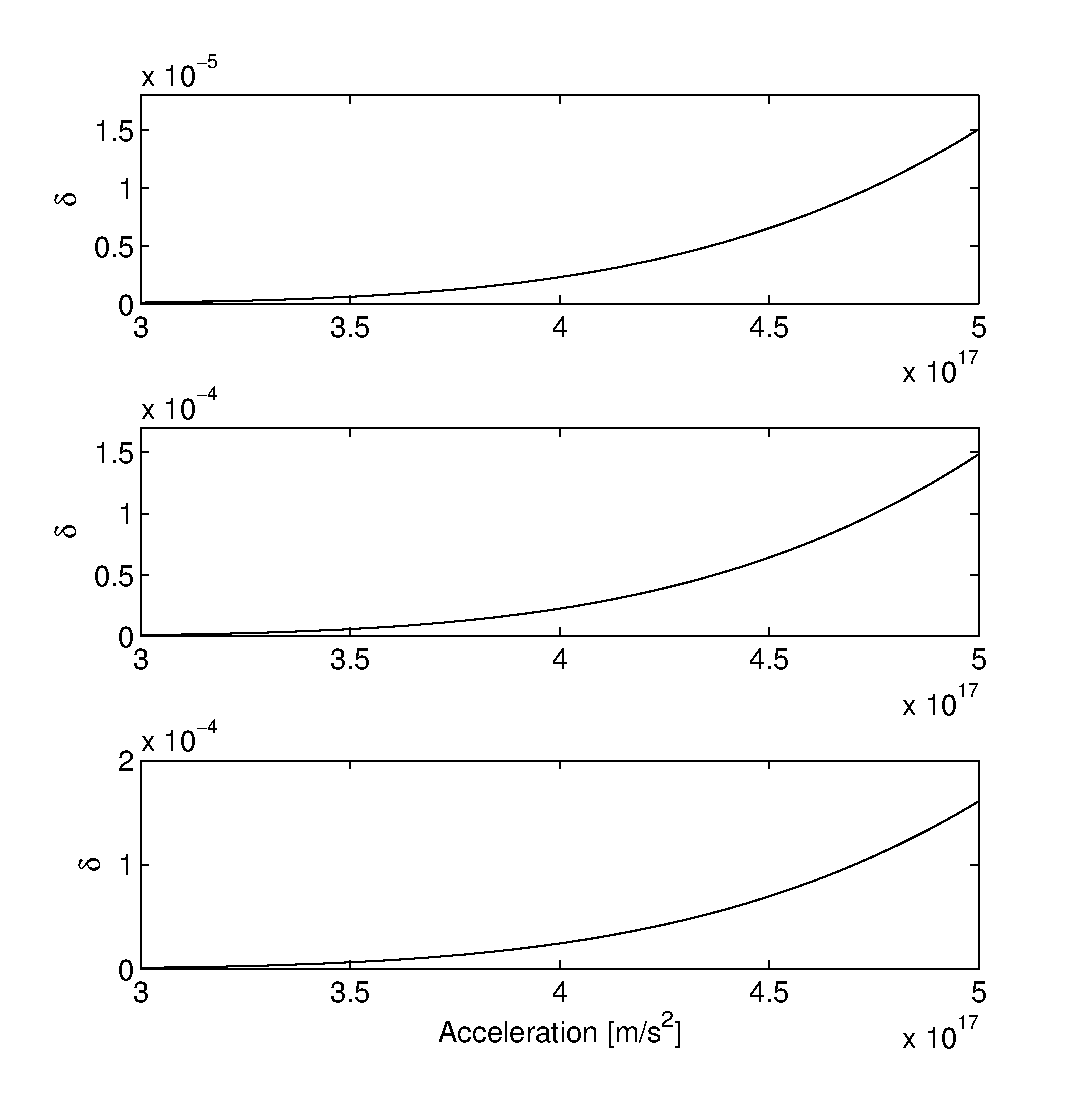
\includegraphics[width=.75\textwidth]{deph}
\caption{$\delta$ for each cycle as a function of the acceleration for three different scenarios. First scenario (top): $\Omega_a\simeq 2.0$ GHz  $\Omega_b\simeq 2.0$ GHz $\lambda\simeq$ 34  Hz.
Second scenario (middle): $\Omega_a\simeq 2.0$ GHz  $\Omega_b\simeq 2.0$ GHz  $\lambda\simeq$  0.10  KHz.
Third scenario (bottom): $\Omega_a\simeq 2.0$ GHz  $\Omega_b\simeq 2.0$ GHz  $\lambda\simeq$ 0.25  KHz.}
\label{deph}
\end{center}
\end{figure}
%\begin{figure}[h]
%\begin{center}
%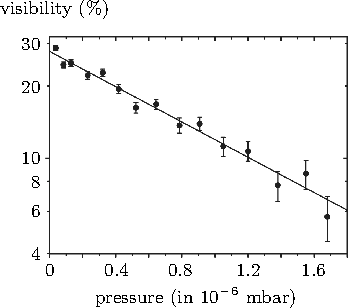
\includegraphics[width=.50\textwidth]{vis}
%\caption{Visibility factor as a function of the acceleration for three different scenarios. First scenario (top): $\Omega_a\simeq 0.10$ THz,  $\Omega_b\simeq 0.16$ THz, $\lambda\simeq 1.5\!\cdot\! 10^{-2}$ THz.
%Second scenario (middle): $\Omega_a\simeq 0.10$ THz  $\Omega_b\simeq 0.12$ THz  $\lambda\simeq  5.5\cdot 10^{-3}$ THz.
%Third scenario (bottom): $\Omega_a\simeq 0.10$ THz  $\Omega_b\simeq 0.10$ THz  $\lambda\simeq 2.5\cdot 10^{-3}$ THz.}
%\label{realf}
%\end{center}
%\end{figure}

The Berry phase acquired by an eigenstate of a system is always a global phase. In order to detect the phase, it is necessary to prepare an interferometric experiment. Indeed, considering a detector in a superposition of an inertial and accelerated trajectory would allow for the detection of the phase. In this context, any experimental set-up in which such a superposition can be implemented would serve our purposes. A possible scenario can be found in the context of atomic interferometry, technology that has already been successfully employed to measure with great precision general relativistic effects such as time dilation due to Earth's gravitational field \cite{atomGR}.

Consider the detector to be an atom which is introduced into an atomic interferometer after being prepared in its ground state. In one arm of the interferometer we let the atom move inertially while in the other arm we consider a mechanism  which produces a uniform acceleration of the atom. Such mechanism could consist of laser pulses that should be prolonged for fractions of nanoseconds.  Such laser technology to produce high accelerations is already available \cite{laser}.  Reaching the desired accelerations is technologically feasible -- however  the detector must survive such accelerations, at least long enough to conclude the interference experiment. For this, the laser pulses must be engineered to create the deep potential wells necessary to accelerate the atom transferring only kinetic energy without exciting it.  As long as the atom does not collide with other atoms this seems feasible \cite{ruso}.  An alternative to this is to consider ions or atomic nuclei as detectors which can be accelerated by applying a potential difference in one arm of the interferometer.  Although the suggested experimental set-up is obviously not exempt from technical difficulties, the problems derived from the experimental challenges involved are expected to be solvable with  present or near-future technology.  


\section{Dynamical phase control}

To measure the Berry phase the relative dynamical phase between the inertial and accelerated paths must be cancelled. In principle the dynamical phase can be controlled and cancelled in any experimental setup. The way to do this depends on the specific experiment considered. 
Fortunately, there is considerable experimental freedom to engineer ways of canceling these phases.  In this section we discuss, as an example, the case of an atomic interferometry experiment. 
 
The control of the dynamical phase boils down to adjusting the relative path length of the interferometer.  Using commercial length metrology equipment it is possible to measure lengths with a precision of $\Delta L\approx 10^{-11}$ m  \footnote{Magnetscale Corporation $\text{Laserscale}^{\text{\textregistered}}$ http://www.gebotech.de/pdf/\\LaserscaleGeneralCatalog\_en\_2010\_04.pdf }.  A detector acquires different dynamical phases when its trajectory is  inertial or accelerated,  therefore the path lengths must be adjusted such that the relative dynamical phase difference cancels or is an integer multiple of $2\pi$.

Since dynamical phases oscillate and geometric ones accumulate, it becomes convenient to let the system evolve through many cycles.  In this way one can make sure that the Berry phase becomes much larger than any precision limit imposed on the length adjustment. If in a given situation the Berry and the dynamical phase differences are of the same order of magnitude, one can consider paths $n$ times longer such that the resulting Berry phase is multiplied by a factor of $n$. 

One can alternatively consider controlling the fly time in the accelerated path by changing the relative velocity of the atoms through the two paths  alternating periods of positive and negative acceleration. In this case, the Berry phase difference adds up (since it always has positive sign). 

In what follows we calculate explicitly with what precision the relative dynamical phase can be controlled.  Consider an atom moving with speed  $v$ (in the laboratory frame) along an inertial trajectory of length $L$. In the case $v\ll c$  the fly time is
$T=L/v$. Changing the path length with a precision of  $\Delta L$ translates to changing the fly time with a precision of
\[\Delta T = \left|\frac{\partial T}{\partial L}\Delta L\right|=\frac{\Delta L}{v}.\]
Since the dynamical phase $\phi$ is proportional to
$\Omega T$,
the resulting precision in adjusting the dynamical phase  is given by
\[\Delta \phi=\Omega \Delta T=\frac{\Omega \Delta L}{v}.\]
Considering for example, $v\approx 100$ m/s, $\Omega\approx 2$ GHz, and  $\Delta L\approx 1 \cdot 10^{-11}$ m we obtain $\Delta \phi=2\cdot10^{-4}$. This precision is enough to distinguish this phase from the Berry phase in a single cycle. The precision can further be increased by adjusting the path length of the accelerated atom.

The speed of the accelerated atom (in the laboratory frame) as a function of proper time is  given by
$v=c\,\tanh\left(\frac{a\tau}{c}\right)$. The path length for the accelerated atom in the laboratory frame $L_a$ is given by the integral of  the speed over proper fly time $T$,
\[L_a=\int_{0}^T c\,\tanh\left(\frac{a\tau}{c}\right) \text{d}\tau=\frac{c^2}{a}\ln\left[\cosh\left(\frac{aT}{c}\right)\right].\]
Therefore, the proper fly time as a function of the path length $L_a$ is
\[ T=c a^{-1}\operatorname{arccosh}\left[\exp\left(\frac{L_a a}{c^2}\right)\right].\]
The precision to control the proper fly time becomes  \[\Delta T=\frac{\Delta L_a}{c}\frac{\exp\left(\frac{L_aa}{c^2}\right)}{\sqrt{\exp\left(\frac{L_aa}{c^2}\right)-1}\sqrt{\exp\left(\frac{L_aa}{c^2}\right)+1}},\]
resulting in a precision to adjusting the dynamical phase of \[\Delta \phi=\Omega \Delta T=\Omega\frac{\Delta L_a}{c}\frac{\exp\left(\frac{L_aa}{c^2}\right)}{\sqrt{\exp\left(\frac{L_aa}{c^2}\right)-1}\sqrt{\exp\left(\frac{L_aa}{c^2}\right)+1}}.\]
\smallskip

For accelerations of $10^{17}$ $\text{m}/\text{s}^2$, $\Omega\approx 2$ GHz,  $\Delta L=10^{-11}$ m and proper lengths $L_a=1$ $\mu$m, $L_a=10$ cm we obtain, respectively\begin{eqnarray}
&\Delta \phi_{L_a=1\mu\text{m}}=2.25\cdot 10^{-8},&\\[3mm]
&\Delta \phi_{L_a=10\text{cm}}=1.49\cdot10^{-10}.&
\end{eqnarray}
We therefore conclude that it is possible to adjust the dynamical phase to several orders of magnitude greater in precision than
that of the Berry phase acquired in a single cycle of adiabatic evolution.

\section{Discussion}

With this proposal to detect the Unruh effect we overcome the difficulties associated with measuring temperatures as small as $10^{-4}$ K. We have shown that the Unruh effect leaves its footprint in the geometric phase acquired by the the joint state of the field and the detector for time scales of about $5\times10^{-10}$ s. The effect is observable for accelerations as low as $10^{17}$ $\text{m}/\text{s}^2$ and can be maximally enhanced by allowing the system to evolve a few microseconds. 

Notice that the Berry phase accumulates in each cycle of adiabatic evolution, and that this is true regardless the sign of the acceleration. This means that in any experiment we could alternate periods of positive and negative acceleration and still the Berry phase will grow, solving the problems of the high relative velocities between atoms going through the two different paths of the interferometer.

Our theoretical setting is general and independent of any particular implementation, paving the way for future experimental proposals. For instance, by considering detector frequencies in the MHz regime,  the method would allow detection of the Unruh effect for accelerations as low as $10^{-14}$ $\text{m}/\text{s}^2$ . For this, other multilevel harmonic systems could be employed as detectors, such as fine structure transitions where frequencies are closer to MHz regime.



